%\section{Computing Continuum}
%\label{sec:example}
%
%%Herein we will discuss the challenges of developing a mobile application that exploits the computing continuum, as well as present a running example that will be used throughout the rest of the paper to exemplify our work.
%
%As previously stated, the continuum enables the convergence of many heterogeneous infrastructures, from cloud-hosted virtual machines down to mobile devices. Given that the two fundamental elements of computation are data and behavior, the first major challenge of developing an application that exploits the computing continuum consists in \emph{deciding where in the continuum the data and the behavior should be deployed}. This decision needs to be informed by the profound heterogeneity that exists between the different infrastructures that constitute the continuum. 
%
%Amongst other things one must take into account important QoS aspects, such as availability and latency, as discussed in Section~\ref{sec:intro}. Let us focus, for example, on a continuum that comprises a cloud-based solution, an edge-based infrastructure, and a mobile device. Data and behavior that are deployed to cloud solutions will benefit from high availability, at the cost of introducing higher latency; while data and behavior deployed to an edge-based infrastructure will benefit from a much lower latency, at the cost of having a lower availability as well. A third possibility would be to deploy the data and the behavior exclusively to the mobile device; however, this could lead to important battery drains (see Section~\ref{sec:evaluation}), not to mention other limitations. Balancing these trade-offs at design time can be difficult. The challenge is, therefore, to allow applications to dynamically, and opportunistically, decide where the data and the behavior should be deployed and executed. 
%
%If we focus on behavior, it is common to distinguish between stateful and stateless computation. The main distinguishing factor between stateful and stateless components is that the latter do not produce side-effects, and that their outputs depend solely on their inputs. If we focus on data, it is common to distinguish between mutable and immutable data. While mutable data can be modified after its creation, the same is not true for immutable data. In components that adopt immutable data, the data is initialized once and for all at deployment time.
%
%As we shall discuss in Section~\ref{sec:proposal}, it is our view that the computing continuum should focus on stateless computation with immutable data. Stateless computation with immutable data is much easier to replicate (and test) across the continuum, since no data synchronization is required and any data needed by the computation can be obtained at deployment time. Nevertheless, stateful computation and mutable data cannot always be excluded entirely from modern applications. For these cases we envision a mixed solution in which traditional cloud-based resources are adopted alongside the continuum. 
%
%Developing applications in the computing continuum also poses other important challenges. For example, when selecting where a certain computation should be achieved, we need to take into account important \emph{security} aspects, such as \emph{authorization}, \emph{confidentiality}, and \emph{integrity}. Also, deployment and execution in the continuum will need \emph{tool} support, e.g., for performing \emph{integration tests}, \emph{runtime monitoring and adaptation}, etc. 
%
%Although these challenges are interesting, and important research endeavors in themselves, in this paper we focus on establishing the basis upon which the computing continuum can develop. In particular, we focus on achieving (i) the dynamic and automatic deployment of computation by part of the infrastructures that constitute the continuum, and (ii) the opportunistic selection of where to execute the computation.

%END OF PREVIOUS CONTINUUM

%REVISED CONTINUUM

\section{The Continuum Model}\label{sec:continuum}

\begin{figure}[tbp]
	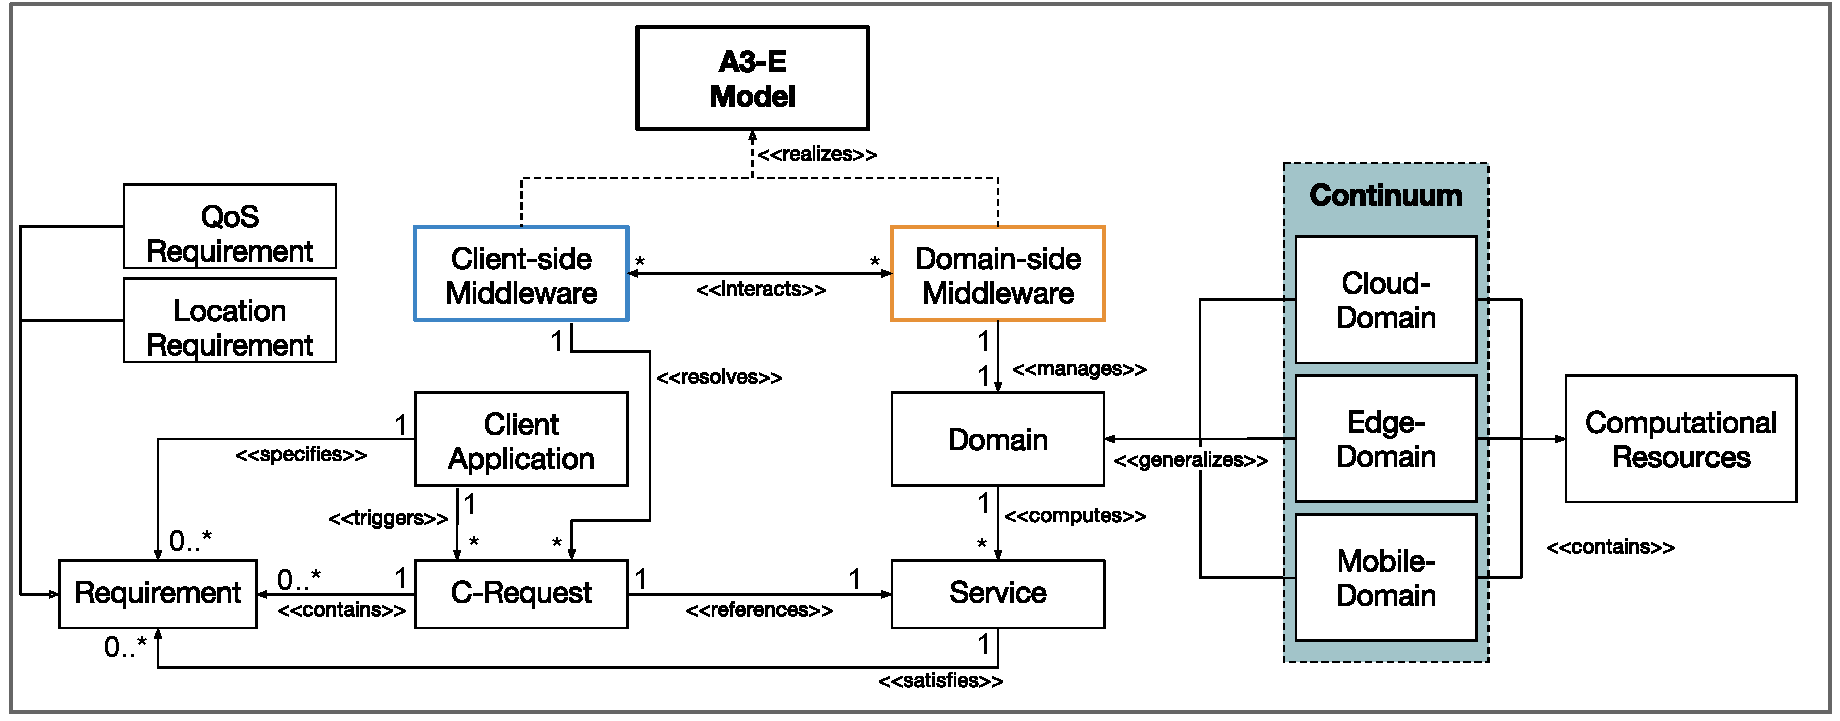
\includegraphics[width=1\textwidth]{figs/A3-E-model.pdf}
	\caption{The Continuum Model.}
	\label{fig:Continuum-model}
\end{figure}

%The \textit{Continuum model}, depicted in Figure~\ref{fig:Continuum-model}, defines the actors and mechanisms involved in the realization of the mobile-edge-cloud continuum.

%Domain formalization
%Application Requirements
%Service SLA
%Service Life-cycle

\subsection{Physical Model}

%Although the continuum can hypothetically support any number of heterogeneous infrastructures, this paper focuses on three domains. The \texttt{mobile domain} is deployed to the client's mobile device, and provides local stateless computation (while enabling device-to-device collaboration through distributed mobile domains --i.e., by allowing a client to call a microservice deployed on another mobile device-- is surely interesting, for now we consider it part of our future work). The \texttt{edge domains} refer to edge-based infrastructure that can be deployed to a local server (local-edge domain) or to cellular stations (mobile-edge domain). Finally, the \texttt{cloud domain} refers to a cloud-based solution such to AWS Lambda.

The continuum is composed of computational resources from cloud, edge, and mobile computing devices. 

Cloud datacenters count with virtually unlimited computational resources needed to cope with the aggregated demand from a wide coverage area. Edge nodes~\footnote{We adopt the more common \textit{node} terminology in detriment of edge datacenters to empathize the fine grained nature of edge computing.}, in contrast, are limited in computational resources, but cover a much narrower area with lower aggregated demand. 

Cloud datacenters are reachable through multiple hops of network, including the Internet backbone. Edge nodes, in turn, are ideally placed a few hops away from clients to minimize network latency and jitter. The continuum model further distinguishes between mobile- and local-edge after the networking technology used: mobile-edge (also known as Multi-access Edge Computing or MEC~\cite{}) integrates with cellular network infrastructure, whereas local-edge integrates with local area network infrastructure. Later on, this heterogeneity is addressed with variations of the proposed service life-cycle management.

In the continuum, mobile devices play two roles: they are clients of continuum services; and they are potential providers. The motivation for the inclusion of mobile devices own resources in the model is threefold: i) the substantial increase in computational capacity of modern devices; ii) the compatibility of these devices to host the execution of continuum functions (see Section~\ref{sec:application_model}); and iii) to give mobile applications a zero network latency and highly available alternative to cloud and edge providers. 

Figure X illustrates a topology composed of cloud, mobile-edge, local-edge, and mobile \textit{domains}. A domain yields a common abstraction for the heterogeneous computational resources (e.g., server(s), virtual machine(s), container(s), memory, CPU, storage, etc.) and networking infrastructure resources (e.g., access points, radio access networks, etc.) composing the continuum.


%constituents of the continuum. Indeed, it hides the fact that they make use of heterogeneous \textit{computational resources} (e.g., server(s), virtual machine(s), container(s), memory, CPU, storage, etc.) and networking infrastructures (e.g., access points, radio access networks, etc.). 

%Examples of A3-E domains are \textit{cloud domains}, i.e., cloud-based FaaS platforms covering a specific geographical region (e.g., AWS Lambda\footnote{\url{https://aws.amazon.com/lambda}} in Europe); \textit{edge domains}, representing local-edge (e.g., domestic servers or within an office building) and mobile-edge sites (e.g., servers at cellular base stations~\cite{beck2014mobile}); and \textit{mobile domain} representing a client device's own resources.

%TODO


%Whilst cloud and edge resources are shared among different applications and managed by cloud/edge providers, mobile device resources are exclusively employed by local applications. 

\subsection{Application Model}\label{sec:application_model}

\begin{figure}[tbp]
	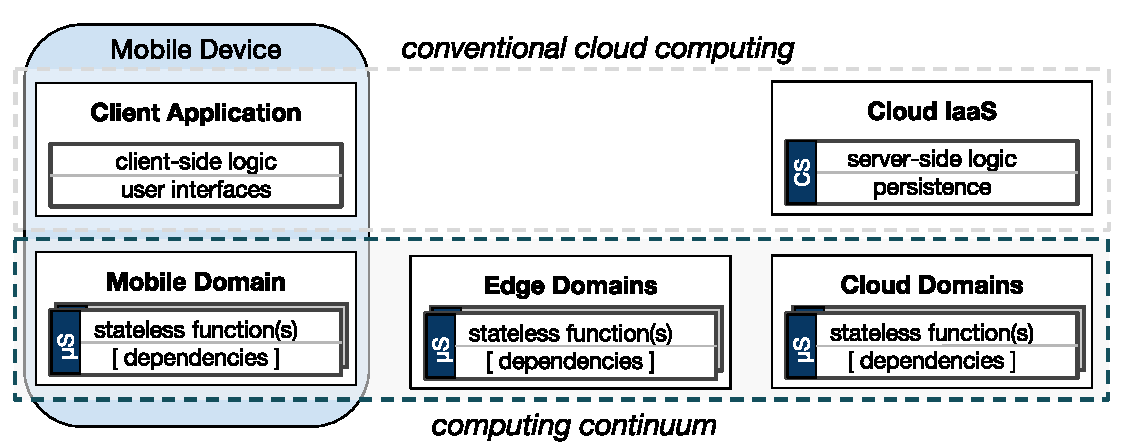
\includegraphics[width=0.9\textwidth]{figs/Continuum-arch}
	\caption{The high level architecture of a mobile application exploiting both the computing continuum -- by means of microservices ($\mu$S) provided by mobile, edge, and cloud domains -- and conventional cloud computing -- by means of cloud services (CS).}
	\label{fig:Continuum-arch}
\end{figure}

We propose an application model in which stateless components and immutable data composing \textit{continuum services} are dynamically placed to mobile, edge, and cloud
whilst 
stateful components are deployed to cloud datacenters or the client device itself after application specific design decisions.

Continuum services consist of a set of artifacts that fulfill a given functionality. In particular, these artifacts can refer to: (i) stateless function(s) (e.g., a Java compiled class); (ii) immutable data (e.g., a trained neural network model); and (iii) other dependencies (e.g., software libraries).

Continuum services should be portable, unless they require capabilities that can not be met by specific domains. Moreover, these services are \textit{microservices}~\cite{lewis2014microservices}, as they are small, modular, communicate with lightweight mechanisms (often through an HTTP RESTful API) and are independently deployable by fully automated machinery. %Accordingly, hereinafter we refer to continuum microservices.
Like cloud and edge domains, mobile domains also expose functionality by means of a well-known interface. For the sake of simplicity, the term microservice is employed with all domains.

%TODO: make it more general, as some applications may have local persistence 
Figure~\ref{fig:Continuum-arch} illustrates the architecture overview of a continuum application that exploits both the continuum and conventional cloud infrastructure (IaaS). The client application comprises \texttt{client-side logic} and \texttt{graphical user interfaces}. While the cloud infrastructure is used for \texttt{server-side logic} and for \texttt{persistence}, the continuum is used for stateless computation, provided by \texttt{stateless functions} that are exposed as \texttt{microservices}.  

The proposed model enforces consistency and allows multiple instances of continuum services to coexist in different parts of the continuum. Also, service instances may be deployed and undeployed independently without the need for state migration, favoring the seamlessly transition from one service provider to the other. The latter is particularly important to cope with the mobility of clients.

As state is a fundamental aspect of many applications, we argue that mobile devices and, for most cases, cloud datacenters should remain responsible for stateful components such as databases. This choice prevents the consistency problems (and the corresponding complexity of potential solutions) that would arise if databases were deployed to finely distributed edge nodes. Moreover, this decision is aligned with the limitations in computational resources of edge nodes. %Indeed, the deployment of components like databases to the edge would be unrealistic for large scale applications.



\subsection{Running Example}
\label{sub:example}

%Throughout this section an example scenario (Fig.~\ref{fig:continuum-scenario}) is used to illustrate the use of A3-E model and the cloud-edge-mobile continuum with different applications employed by a person with visual impairment.
%We shall now introduce the running example that will be used throughout the rest of the paper. 
Figure~\ref{fig:continuum-scenario} shows a complete example scenario that starts in a user's office and finishes at her home. It involves different applications that rely on computation executed in the cloud, edge, or in the user's own devices. 

First, let us assume the existence of a local edge server in the user's office (hereafter called \textit{local-edge}). This server is owned by the company, and it is used to extend the computational capabilities of the devices operated by its employees. In our example, the user makes use of an augmented reality (AR) application to craft virtual 3D objects that are added to her desk table. This application involves heavyweight image processing for the \textit{extraction of features} from the captured scenes, as well as a trained neural network model to \textit{detect objects} from a set of features. With the offloading of both tasks to the local-edge, the user can avoid recharging her glasses and can improve her productivity. Also, the additional storage on the edge servers allows a larger set of objects to be recognized, thanks to a more completely trained model.

\begin{figure}[tbp]
	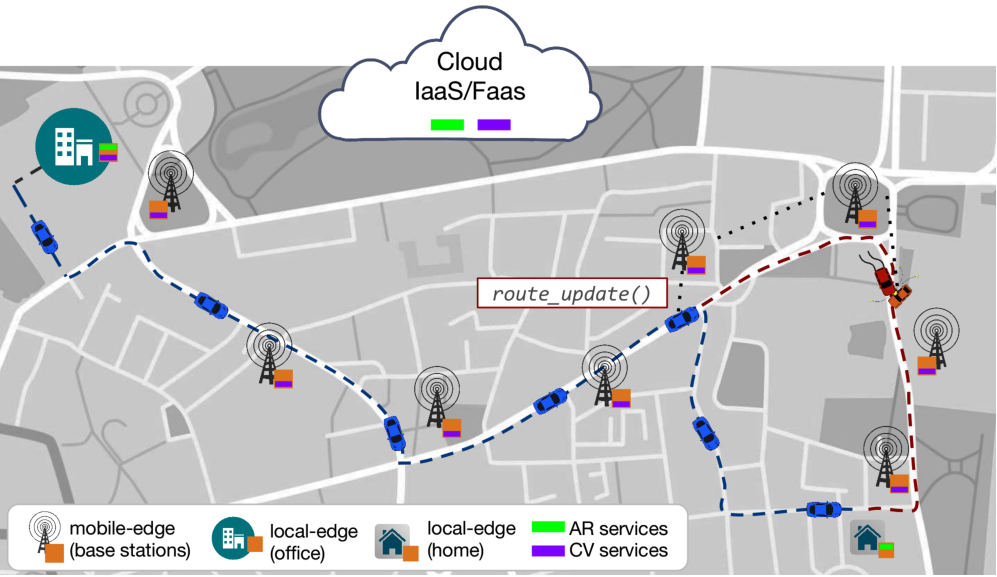
\includegraphics[width=0.9\textwidth]{figs/Continuum-Scenario}
	\caption{Heterogeneous applications such as Augmented Reality (AR), Autonomous Vehicles (AV) and Mobile Games (MG) interact with services deployed along the computing continuum (cloud, mobile-edge, local-edge, and mobile)}
	\label{fig:continuum-scenario}
\end{figure}

After work, the user leaves her offices and enters her autonomous vehicle (AV). During her way home, the vehicle makes use of microservices deployed at edge servers located at cellular base stations (hereafter called \textit{mobile-edge}) to receive low-latency updates about the best plan to reach her destination. This way, within milliseconds the vehicle can be suggested to adjust its routes to avoid heavy traffic. In particular, let's say that a new path consists of residential streets with data services only (without mobile-edge coverage). The AV continues to fetch updates, which are now served by a cloud provider. The additional network latency is partially compensated with the low speed limit of the residential area.

During our user's journey home, her AV passes by a touristic region. The mobile-edge stations covering this area feature services to be consumed by an AR application for tourists. These services share computational resources with those serving autonomous vehicles passing by the touristic area, as well as any other services provided by the aforementioned mobile-edge stations.

Finally, at home the user can start using her domestic local-edge server. She finds out about a new Mobile Game (MG) application. Upon installation, the local-edge server becomes aware of a new continuum-compliant application and, while the app continues to run locally on her device, it proceeds to setup the services needed to allow the application to offload some of the computation. Once the setup is complete, the application autonomously starts using the edge services with the purpose of preserving the device's resources. Not only does the game's performance improve, battery consumption is also reduced.  

This scenario exploits different parts of the continuum. Traditional cloud resources are employed as a reliable alternative to edge-based computation. Similarly, local services are employed as alternatives to edge services until they have been acquired and made available by a local-edge server. Whilst the transition between mobile-edge and cloud is transparent, the use of local-edge services involves mutual client-server awareness.

%TODO Merge below
%Considering our running example, the office AR application consists of a client-side logic responsible for capturing scenes from the glasses' camera and microservices in the continuum that extract features from objects in the scene (e.g., the user's desk, hands, crafting tools) based on an image processing library and a neural network trained model. Client-side logic is then responsible for updating the 3D virtual object state and rendering it into the scene displayed by the glasses.

%The mobile game application, in turn, consists of client-side logic and user interfaces (e.g., controllers and views of an MVC model~\footnote{Model-View-Controller}). The continuum provides the logic for processing and updating the game state, which must be passed as a parameter to a microservice in the continuum, in conjunction with game events (e.g., user inputs). Finally, cloud services provide stateful server-side logic (e.g. authentication, business logic) and persistence (e.g., player scores). 
